\section{Experiments}
\label{sec:experiments}

\subsection{Protocol}

We evaluate six systems on the frozen \textsc{eval\_v1} split: two non-LLM
baselines and four reasoning-effort configurations across two frontier
multimodal models. Exact invocation details are provided in
Appendix~\ref{app:reproducibility}.
\begin{itemize}
  \item \textbf{Empty-Program} -- a floor baseline that always predicts an empty
    string; every sample fails parsing.
  \item \textbf{Heuristic-CV} -- a classical-CV baseline that thresholds the
    image, labels connected components, classifies each component as a circle or
    square by bounding-box fill ratio, and as hollow or filled by morphological
    erosion. Stroke widths are estimated from the ratio of component area to
    estimated perimeter.
  \item \textbf{\textsc{Claude Opus 4.7} (1M context)} at \texttt{high} and
    \texttt{max} effort.
  \item \textbf{\textsc{GPT-5.5}} at \texttt{medium} and \texttt{extra\_high}
    reasoning effort.
\end{itemize}

All four LLM configurations share the same zero-shot prompt: a one-sentence
system instruction (``Return only valid ui-bench DSL code. Do not include
markdown fences, comments, or prose.'') and a user block listing the four
primitive signatures and formatting constraints. We do not use chain-of-thought
prompting or few-shot examples. Raw model outputs are post-processed by a shared
normalizer that prefers fenced code blocks anywhere in the response, falls back
to primitive-signature line filtering, and ultimately surfaces the raw response
so that parse errors are visible rather than masked.

\subsection{Runner and artifacts}

Each run writes a per-run directory under \texttt{data/runs/} containing
\texttt{run\_config.json}, \texttt{summary.json}, and per-sample JSON files with
the request, raw and normalized predictions, usage, latency, and the full
evaluation result. All metrics in this paper are computed from these artifacts by
\texttt{scripts/analyze.py}; figures are produced by
\texttt{scripts/make\_figures.py}. We use non-parametric bootstrap with 1000
resamples for 95\% confidence intervals on per-difficulty means.

\subsection{Headline results}

Table~\ref{tab:main-results} reports the aggregated metrics across all 150
samples for each system; 95\% bootstrap CIs are shown in brackets.
Figure~\ref{fig:acc-by-diff} breaks the exact-match rate down by difficulty
tier, and Figure~\ref{fig:metric-panel} shows the same decomposition for all
four scored metrics.

\begin{table}[!htbp]
  \centering
  \small
  % Auto-generated by scripts/analyze.py. Do not edit by hand.
\begin{tabular}{lrrrr}
\toprule
Model & Exact & PixAcc & FG-IoU & Parse \\
\midrule
Heuristic-CV & 0.087 {\scriptsize [0.047, 0.133]} & 0.881 {\scriptsize [0.862, 0.898]} & 0.583 {\scriptsize [0.535, 0.628]} & 1.000 {\scriptsize [1.000, 1.000]} \\
gpt-5.5 (medium) & 0.027 {\scriptsize [0.007, 0.053]} & 0.963 {\scriptsize [0.937, 0.984]} & 0.850 {\scriptsize [0.813, 0.884]} & 0.973 {\scriptsize [0.947, 0.993]} \\
gpt-5.5 (extra\_high) & 0.020 {\scriptsize [0.000, 0.040]} & 0.983 {\scriptsize [0.969, 0.991]} & 0.865 {\scriptsize [0.836, 0.893]} & 0.993 {\scriptsize [0.980, 1.000]} \\
Empty-Program & 0.000 {\scriptsize [0.000, 0.000]} & 0.000 {\scriptsize [0.000, 0.000]} & 0.000 {\scriptsize [0.000, 0.000]} & 0.000 {\scriptsize [0.000, 0.000]} \\
claude-opus-4-7[1m] (high) & 0.000 {\scriptsize [0.000, 0.000]} & 0.900 {\scriptsize [0.873, 0.919]} & 0.439 {\scriptsize [0.403, 0.474]} & 0.980 {\scriptsize [0.960, 1.000]} \\
claude-opus-4-7[1m] (max) & 0.000 {\scriptsize [0.000, 0.000]} & 0.919 {\scriptsize [0.912, 0.927]} & 0.461 {\scriptsize [0.427, 0.495]} & 1.000 {\scriptsize [1.000, 1.000]} \\
\bottomrule
\end{tabular}

  \caption{Main results on \textsc{eval\_v1}. ``Exact'' is pixel-exact raster
  match; ``PixAcc'' is mean pixel accuracy; ``FG-IoU'' is mean foreground IoU;
  ``Parse'' is parse success rate. Brackets give 95\% bootstrap CIs.}
  \label{tab:main-results}
\end{table}

\begin{figure}[!htbp]
  \centering
  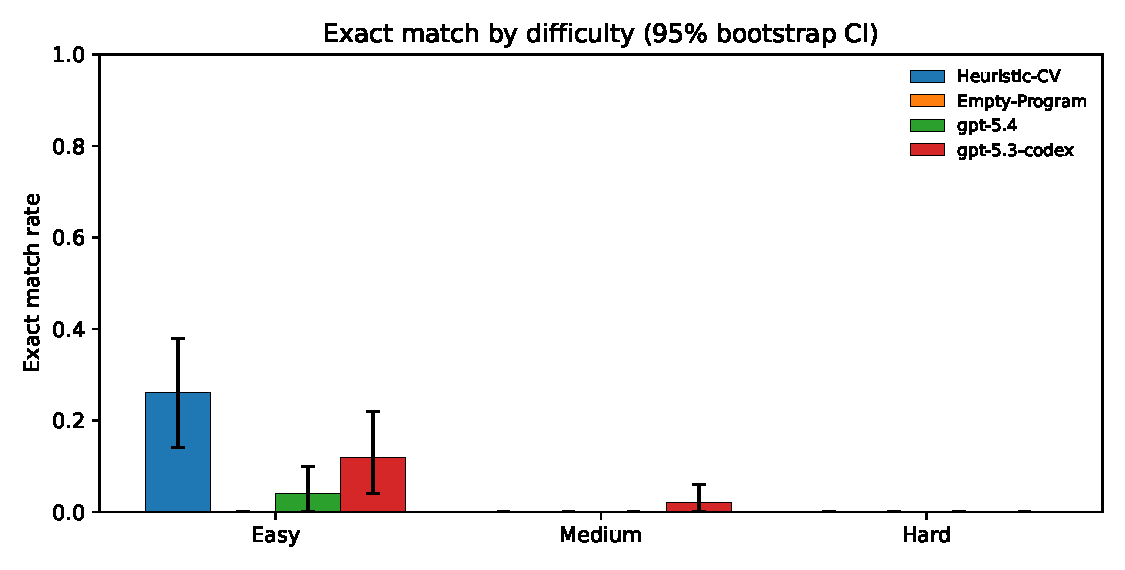
\includegraphics[width=\linewidth]{figures/fig_accuracy_by_difficulty.pdf}
  \caption{Exact-match rate by difficulty tier. Error bars are 95\% bootstrap
  CIs over per-sample indicators.}
  \label{fig:acc-by-diff}
\end{figure}

\begin{figure}[!htbp]
  \centering
  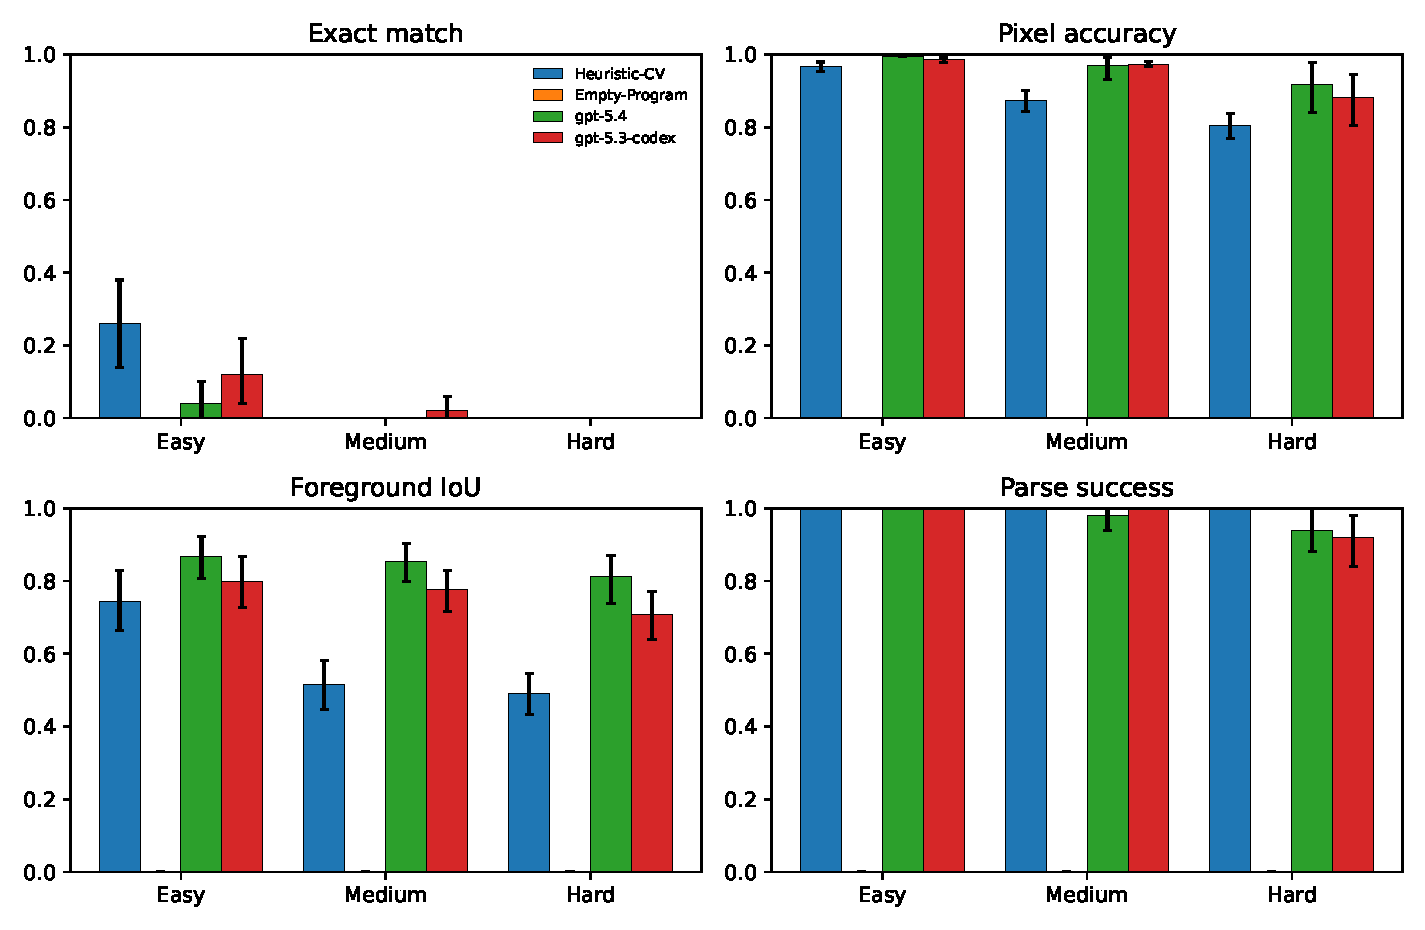
\includegraphics[width=\linewidth]{figures/fig_metric_comparison.pdf}
  \caption{All four scored metrics by difficulty tier. The four panels are
  exact-match, pixel accuracy, foreground IoU, and parse success.}
  \label{fig:metric-panel}
\end{figure}

The key qualitative pattern -- detailed in Section~\ref{sec:analysis} -- is that
exact-match collapses on the hard tier for every system, while
foreground IoU degrades more gracefully; the heuristic baseline is surprisingly
competitive on easy scenes and is outclassed on hard scenes, where LLMs can
enumerate and place multiple overlapping shapes that classical connected
components cannot individuate.
